\item \points{30} {\bf Incomplete, Positive-Only Labels}

In this problem we will consider training binary classifiers in situations
where we do not have full access to the labels. In particular, we consider
a scenario, which is not too infrequent in real life, where we have labels
only for a subset of the positive examples. All the negative examples and
the rest of the positive examples are unlabelled.

We formalize the scenario as follows. Let $\{(x^{(i)}, t^{(i)})\}_{i=1}^\nexp$ be a standard dataset of i.i.d distributed examples. Here $x^{(i)}$'s are the inputs/features and $t^{(i)}$ are the labels. Now consider the situation where $t^{(i)}$'s are not observed by us. Instead, we only observe the labels of some of the positive examples. Concretely, we assume that we observe  $y^{(i)}$'s that are generated by
\begin{align*}
& \forall  x, ~~ p(y^{(i)} = 1\mid t^{(i)}=1, x^{(i)}=x) = \alpha, \\
& \forall  x, ~~ p(y^{(i)} = 0 \mid t^{(i)}=1, x^{(i)}=x)  = 1- \alpha\\
& \forall  x, ~~ p(y^{(i)} = 1 \mid t^{(i)}=0, x^{(i)}=x) = 0,\\ 
& \forall  x, ~~ p(y^{(i)} = 0 \mid t^{(i)}=0, x^{(i)}=x) = 1
\end{align*}
where $\alpha \in (0,1)$ is some unknown scalar. In other words, if the unobserved ``true'' label $t^{(i)}$ is 1, then with $\alpha$ chance we observe a label $y^{(i)} = 1$. On the other hand, if the unobserved ``true'' label $t^{(i)} = 0$, then we always observe the label $y^{(i)} = 0$. 

Our final goal in the problem is to construct a binary classifier $h$ of
the true label $t$, with only access to the partial label $y$. In other words,
we want to construct $h$ such that
 $h(x^{(i)}) \approx p(t^{(i)} = 1\mid x^{(i)})$ as closely as
possible, using only $x$ and $y$.

\emph{Real world example: Suppose we maintain a database of proteins which
are involved in transmitting signals across membranes. Every example added to
the database is involved in a signaling process, but there are many proteins
involved in cross-membrane signaling which are missing from the database.
It would be useful to train a classifier to identify proteins that
should be added to the database. In our notation, each example $x^{(i)}$
corresponds to a protein, $y^{(i)} = 1$ if the protein is in the database and
$0$ otherwise, and $t^{(i)} = 1$ if the protein is involved in a cross-membrane
signaling process and thus should be added to the database, and $0$ otherwise.}


For the rest of the question, we will use the dataset and starter code provided in
the following files:
%
\begin{center}
\begin{itemize}
\item	\url{src/posonly/{train,valid,test}.csv}
\item   \url{src/posonly/posonly.py}
\end{itemize}
\end{center}
%
Each file contains the following columns: $x_1$, $x_2$, $y$, and $t$. As in
Problem 1, there is one example per row. The $y^{(i)}$'s are generated from the process defined above with some unknown $\alpha$.


\begin{enumerate}
        \item \subquestionpoints{5} \textbf{Coding problem: ideal (fully observed) case}

First we will consider the hypothetical (and uninteresting) case, where we have access to the true
$t$-labels for training. In \texttt{src/posonly/posonly.py}, write a logistic
regression classifier that uses $x_1$ and $x_2$ as input features, and train it
using the $t$-labels. We will ignore the $y$-labels for this part. Output the
trained model's predictions on the \textbf{test set} to the file specified in the code.

Create a plot to visualize the test set with $x_1$ on the horizontal axis and $x_2$ on
the vertical axis. Use different symbols for examples $x^{(i)}$ with true label $t^{(i)} = 1$
than those with $t^{(i)} = 0$. On the same figure, plot the decision boundary obtained
by your model (i.e, line corresponding to model's predicted probability = 0.5) in red color. Include
this plot in your writeup.



        \ifnum\solutions=1 {
	  \begin{answer}
	\begin{figure*}[h]
	    \centering
	    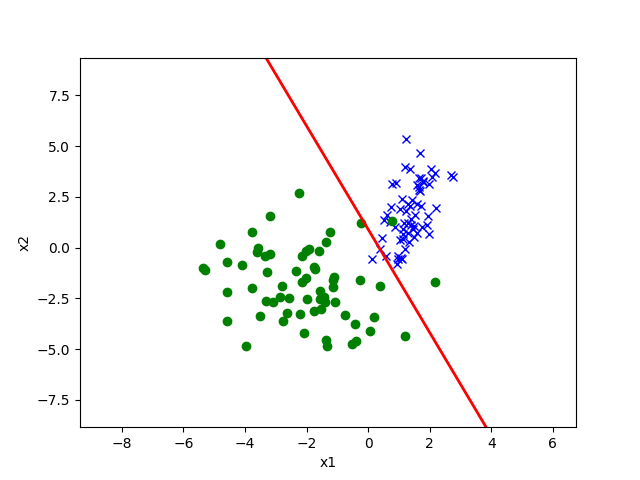
\includegraphics[width=0.5\linewidth]{tex/posonly/posonly_true_pred.png}
	    \caption{Train theta to t, and test on t}
	    \label{fig:my_label}
	\end{figure*}
\end{answer}

        }\fi

        \item \subquestionpoints{5} \textbf{Coding problem: The naive method on partial labels}

We now consider the case where the $t$-labels are unavailable, so you only have
access to the $y$-labels at training time. Extend your code in
\texttt{src/posonly/posonly.py} to re-train the classifier (still using $x_1$ and
$x_2$ as input features), but using the $y$-labels only. Output the predictions
on the \textbf{test set} to the appropriate file (as described in the code comments).


Create a plot to visualize the test set with $x_1$ on the horizontal axis and $x_2$ on
the vertical axis. Use different symbols for examples $x^{(i)}$ with true label $t^{(i)} = 1$ (even though we only
used the $y^{(i)}$ labels for training, use the true $t^{(i)}$ labels for plotting)
than those with $t^{(i)} = 0$. On the same figure, plot the decision boundary obtained
by your model (i.e, line corresponding to model's predicted probability = 0.5) in red color. Include
this plot in your writeup.


Note that the algorithm should learn a function $h(\cdot)$ that approximately predicts the probability $p(y^{(i)}=1\mid x^{(i)})$. Also note that we expect it to perform poorly on predicting the probability of interest, namely $p(t^{(i)}=1\mid x^{(i)})$.


        \ifnum\solutions=1 {
	  \begin{answer}
	\begin{figure*}[h!]
	    \centering
	    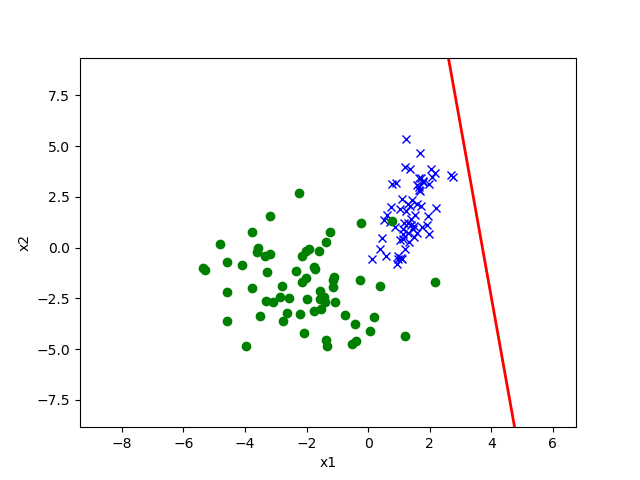
\includegraphics[width=0.35\linewidth]{tex/posonly/posonly_naive_pred.png}
	    \caption{Train theta to y, and test on t}
	    \label{fig:my_label}
	\end{figure*}

\end{answer}

        } \fi

        \vspace{0.3in}
In the following sub-questions we will attempt to solve the problem with only partial observations. That is, we only have access to $\{(x^{(i)}, y^{(i)})\}_{i=1}^n$, and will try to predict $p(t^{(i)}=1 | x^{(i)})$.

\item \subquestionpoints{5} \textbf{Warm-up with Bayes rule}

Show that under our assumptions, for any $i$, 
\begin{align}
p(t^{(i)}=1\mid y^{(i)} = 1, x^{(i)}) = 1
\end{align}
That is, observing a positive partial label $y^{(i)}=1$ tells us for sure the hidden true label is 1. Use Bayes rule to derive this (an informal explanation will not earn credit).


        \ifnum\solutions=1 {
	  \begin{answer}
\begin{align*}
  p(t^{(i)}=1|y^{(i)}=1,x^{(i)})&=\dfrac{p(y^{(i)}=1|t^{(i)}=1,x^{(i)})p(t^{(i)}=1|x^{(i)})}{p(y^{(i)}=1|x^{(i)})}\\
  &=\dfrac{p(y^{(i)}=1|t^{(i)}=1,x^{(i)})p(t^{(i)}=1|x^{(i)})}{p(y^{(i)}=1|t^{(i)}=0,x^{(i)})p(t^{(i)}=0|x^{(i)}) +  p(y^{(i)}=1|t^{(i)}=1,x^{(i)})p(t^{(i)}=1|x^{(i)})}\\
  &=\dfrac{p(y^{(i)}=1|t^{(i)}=1,x^{(i)})p(t^{(i)}=1|x^{(i)})}{0 \cdot p(t^{(i)}=0|x^{(i)}) +  p(y^{(i)}=1|t^{(i)}=1,x^{(i)})p(t^{(i)}=1|x^{(i)})}\\
  &=\dfrac{p(y^{(i)}=1|t^{(i)}=1,x^{(i)})p(t^{(i)}=1|x^{(i)})}{p(y^{(i)}=1|t^{(i)}=1,x^{(i)})p(t^{(i)}=1|x^{(i)})}\\
  &=1
\end{align*}
\end{answer}

        } \fi

	\item \subquestionpoints{5} 
Show that for any example, the probability that true label $t^{(i)}$ is positive is $1/\alpha$ times  the probability that the partial label is positive. 
That is, show that
\begin{align}p(t^{(i)} = 1\mid x^{(i)}) = \frac{1}{\alpha}\cdot p(y^{(i)} = 1\mid x^{(i)})\label{eqn:3} \end{align}

Note that the equation above suggests that if we know the value of $\alpha$, then we can convert a function $h(\cdot)$ that approximately predicts the probability $h(x^{(i)}) \approx p(y^{(i)}=1\mid x^{(i)})$ into a function that approximately predicts $p(t^{(i)} = 1\mid x^{(i)}) $ by multiplying the factor $1/\alpha$. 



        \ifnum\solutions=1 {
	  \begin{answer}
From previous sub-problem, we got...
	\begin{equation*}
	    p(y^{i} = 1, t^{i} = 1, x^{i}) = p(y^{i} = 1, x^{i})
	\end{equation*}
	\begin{equation*}
	    p(y^{i} = 1, t^{i} = 1, x^{i}) = p(y^{i} = 1|t^{i} = 1,x^{i})p(t^{i} = 1|x^{i})p(x^{i}) = \alpha*p(t^{i} = 1|x^{i})p(x^{i})
	\end{equation*}
	\begin{equation*}
	    \alpha*p(t^{i} = 1|x^{i})p(x^{i}) =  p(y^{i} = 1, x^{i}) \Rightarrow p(t^{i} = 1|x^{i}) = \frac{p(y^{i} = 1, x^{i})}{p(x^{i})}*(\frac{1}{\alpha})
	\end{equation*}
	\begin{equation*}
	    \frac{p(y^{i} = 1, x^{i})}{p(x^{i})}*(\frac{1}{\alpha}) = \frac{p(y^{i} = 1|x^{i})}{\alpha}
	\end{equation*}
	
	Therefore, 
	\begin{equation*}
	p(t^{(i)} = 1\mid x^{(i)}) = \frac{1}{\alpha}\cdot p(y^{(i)} = 1\mid x^{(i)})\label{eqn:3} 
	\end{equation*}
	
\end{answer}

        } \fi

	\item \subquestionpoints{5} \textbf{Estimating $\alpha$}


The solution to estimate $p(t^{(i)}|x^{(i)})$ outlined in the previous sub-question requires the knowledge of $\alpha$ which we don't have. Now we will design a way to estimate $\alpha$ based on the function $h(\cdot)$ that approximately predicts $p(y^{(i)}=1\mid x^{(i)})$ (which we obtained in part b).  

To simplify the analysis, let's assume that we have magically obtained a function $h(x)$ that perfectly predicts the value of $p(y^{(i)}=1\mid x^{(i)})$, that is, $h(x^{(i)} )= p(y^{(i)} = 1\mid x^{(i)})$.

We make the crucial assumption that $p(t^{(i)}=1\mid x^{(i)}) \in \{0,1\}$. This assumption means that the process of generating the ``true'' label $t^{(i)}$ is a noise-free process. This assumption is not very unreasonable to make. Note, we are NOT assuming that the observed label $y^{(i)}$ is noise-free, which would be an unreasonable assumption!

Now we will show that:
\begin{align}
\alpha = \mathbb{E}[h(x^{(i)})\mid y^{(i)}=1] \label{eqn:1}
\end{align}
%To show this, prove that $h(x^{(i)}) = \alpha$ when $y^{(i)} = 1$. 

The above result motivates the following algorithm to estimate $\alpha$ by estimating the RHS of the equation above using samples: 
Let $V_{+}$ be the set of labeled (and hence positive) examples in the validation set $V$, given by $V_{+} = \{x^{(i)}\in V\mid y^{(i)} = 1\}$.

Then we use 
\begin{equation*}
\alpha \approx \frac{1}{|V_{+}|}\sum_{x^{(i)}\in V_{+}} h(x^{(i)}).
\end{equation*}
to estimate $\alpha$. (You will be asked to implement this algorithm in the next sub-question. For this sub-question, you only need to show equation~\eqref{eqn:1}. Moreover, this sub-question may be slightly harder than other sub-questions.)


        \ifnum\solutions=1 {
	  \begin{answer}
    Your solution here.

\end{answer}

        } \fi

	\item \subquestionpoints{5} \textbf{Coding problem.}

Using the validation set, estimate the constant $\alpha$ by averaging your
classifier's predictions over all labeled examples in the validation set:\footnote{There is a reason to use the validation set, instead of the training set, to estimate the $\alpha$. However, for the purpose of this question, we sweep the subtlety here under the rug, and you don't need to understand the difference between the two for this question. } 
%
\begin{equation*}
  \alpha \approx \frac{1}{|V_{+}|}\sum_{x^{(i)}\in V_{+}} h(x^{(i)}).
\end{equation*}
%
Add code in \texttt{src/posonly/posonly.py} to rescale your
 predictions $h(y^{(i)}=1\mid x^{(i)})$ of the classifier that is obtained from part b,  using the equation~\eqref{eqn:3} obtained in part (d) and using the estimated value for $\alpha$.



Finally, create a plot to visualize the test set with $x_1$ on the horizontal axis and $x_2$ on
the vertical axis. Use different symbols for examples $x^{(i)}$ with true label $t^{(i)} = 1$ (even though we only
used the $y^{(i)}$ labels for training, use the true $t^{(i)}$ labels for plotting)
than those with $t^{(i)} = 0$. On the same figure, plot the decision boundary obtained
by your model (i.e, line corresponding to model's \textbf{adjusted} predicted probability = 0.5) in red color. Include
this plot in your writeup.


        \ifnum\solutions=1 {
	  \begin{answer}
	\begin{figure*}[h]
	    \centering
	    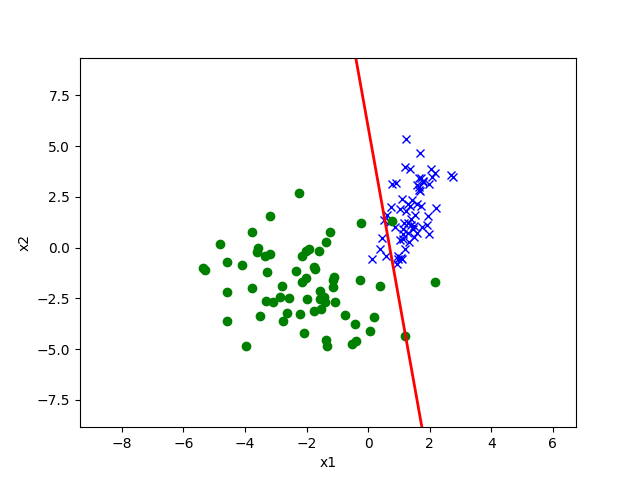
\includegraphics[width=0.5\linewidth]{tex/posonly/posonly_adjusted_pred.png}
	    \caption{Adjusted naive prediction with alpha}
	    \label{fig:my_label}
	\end{figure*}
\end{answer}

        } \fi
\end{enumerate}

\textbf{Remark}: We saw that the true probability $p(t\mid x)$ was only a
constant factor away from $p(y\mid x)$. This means, if our task is to only rank
examples (\emph{i.e.} sort them) in a particular order (e.g, sort the proteins
in order of being most likely to be involved in transmitting signals across
membranes), then in fact we do not even need to estimate $\alpha$. The rank
based on $p(y\mid x)$ will agree with the rank based on $p(t\mid x)$.
